\section{Esimation of cell size.}



\begin{figure}
		\centering
    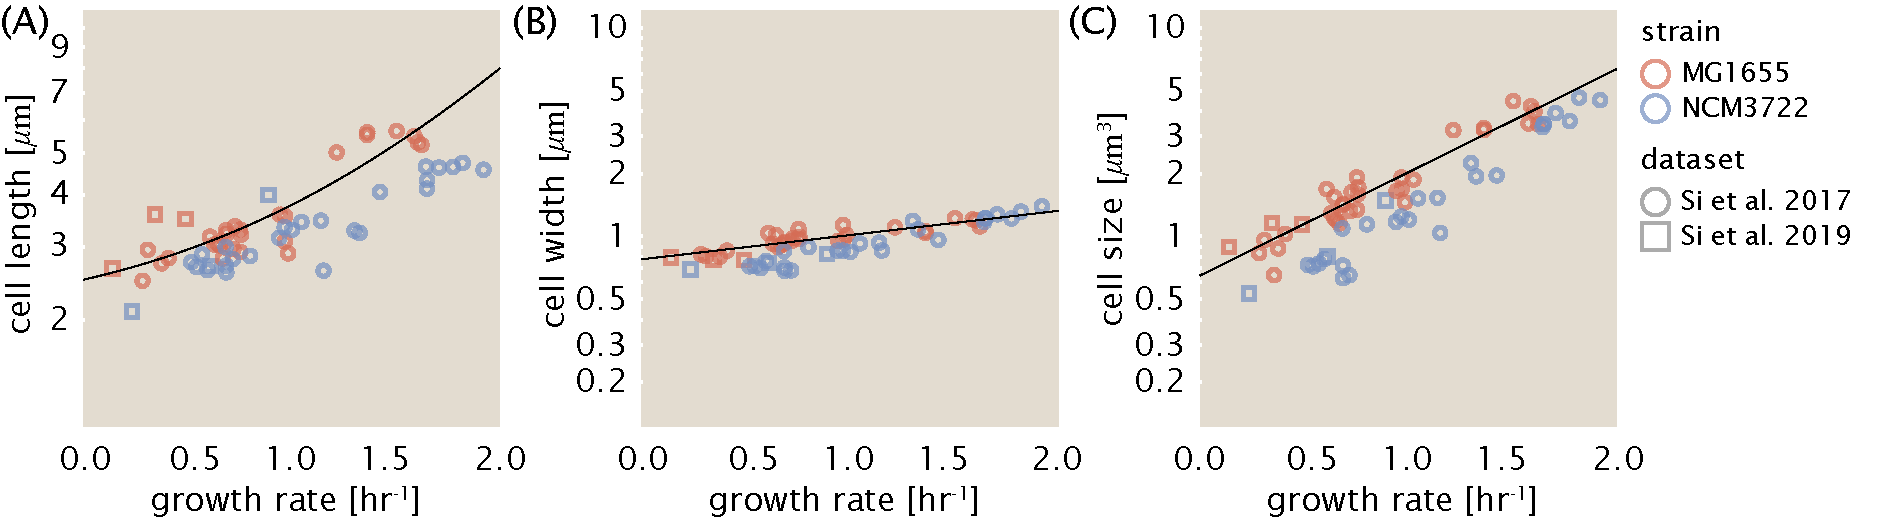
\includegraphics[width=1.0\textwidth]{SI_figs/final_cell_size_Si.pdf}
  \caption{\textbf{Summary of size measurements from Si \textit{et al.} 2017, 2019.}
	 	 Cell lengths and widths were measured from cell contours obtained from
	 	 phase contrast images, and refer to the long and short axis respectively.
	 	 (A) Cell lengths and (B) cell widths show the mean measurements reported
	 	 (they report 140-300 images and 5,000-30,000 for each set of samples;
	 	 which likely means about 1,000-5,000 measurements per mean value reported
	 	 here since they considered about 6 conditions at a time). Fits were made
	 	 to the  MG1655 strain data; length: 0.5 $e^{1.09 \cdot \lambda}$ + 1.76
	 	 $\mu$ m, width:  0.64 $e^{0.24 \cdot \lambda}$ $\mu$ m. (C) Cell size,
	 	 $V$, was calculated as cylinders with two hemispherical ends
     ($V$ = $\pi$ r$^2 \cdot$ ($l$ - $2r/3$)) where $r$ is half the cell width, and $l$ is the cell
	 	 length. The MG1655 strain data gave a best fit of 0.533 $e^{1.037 \cdot \lambda}$ $\mu$ m.}
  \label{fig:final_size_data_Si}
\end{figure}
